\documentclass[12pt,PhD,twoside]{muthesis}
\usepackage{verbatim}
\usepackage{graphicx}
\graphicspath{ {img/} }
\usepackage{hyperref}
\usepackage{subfig}

\usepackage{url} % typeset URL's reasonably
\usepackage{listings}
\usepackage{pdfpages}
\usepackage{tabu}
\usepackage{longtable}
\usepackage{multirow, tabularx}
\usepackage[labelfont=bf]{caption}
\usepackage{natbib}
\usepackage{pslatex} % Use Postscript fonts
\usepackage{amsmath}
\usepackage{amssymb}
\usepackage{bm}
\usepackage{pseudocode}
\DeclareMathOperator*{\argmin}{arg\,min}
\DeclareMathOperator*{\argmax}{arg\,max}
\def\approxprop{%
	\def\p{%
		\setbox0=\vbox{\hbox{$\propto$}}%
		\ht0=0.6ex \box0 }%
	\def\s{%
		\vbox{\hbox{$\sim$}}%
	}%
	\mathrel{\raisebox{0.7ex}{%
			\mbox{$\underset{\s}{\p}$}%
		}}%
	}
\def\hlinewd#1{%
	\noalign{\ifnum0=`}\fi\hrule \@height #1 %
	\futurelet\reserved@a\@xhline} 
\begin{document}
\bibliographystyle{model5-names}

\chapter{Metric learning in pairwise difference space}
\label{apx:adsmetric}

\section*{Introduction}

Constraints on which data points should or should not be grouped together (must-link or cannot-link constraints) can significantly improve the performance of clustering. Most conventional semi-supervised approaches try to minimize must-link distances, maximize cannot-link distances, or to enforce a constant limit on either and optimize the other. They do not make explicit use of the probability distribution of must-link and cannot-link distances. 

Here, we propose a framework for semi-supervised clustering based on projecting the data into a distance space in which distances reflect the linkage probabilities of belonging to the same cluster, using simple probabilistic classifiers trained on the available constraints. The framework can be seen as a novel approach to perform non-linear metric learning using weak supervision in the form of pairwise constraints, in order to improve clustering performance, as pioneered by \citep{xing2002distance}. Although this problem is very similar to metric learning in general, the criterion of interest is often somewhat different: as opposed to optimizing the performance of some classifier as in e.g. \citep{bellet2012similarity}), or for a large margin as in e.g. \citep{weinberger2005distance}, the goal is ensuring that all instances of a cluster are closer under the learned metric than those of different clusters. Furthermore, semi-supervised methods requiring partially labelled instances are not applicable if only pairwise constraints are available. 

We have used this framework to model the structure of spatial representations in human participants in Chapter 5 above, using the information which buildings have or have not been co-represented as the must-link and cannot-link constraints to train a Gaussian Discriminant Analysis (GDA) model in absolute pairwise difference space (see also Chapter 2.5 for the mathematical formulation, and Chapter 5 for the results). 

\section*{Motivation}

For general applicability, non-linear metrics are vital, because of the problem of \textit{multimodality}. When data points forming several groups or `modes' in unweighted feature space actually belong to the same cluster semantically, as indicated by ML constraints, there exists no linear projection able to separate them, and linear methods must inevitably fail. A traditional example is the XOR dataset, consisting of four groups, connected by diagonal ML constraints, such that there exists no linear separating hyperplane - see Figure \ref{fig:motivation}a. 

Although kernel-based methods can deal with multimodal clustering problems (or any complicated data distribution) according to the Representer Theorem, in theory, given the optimal kernel and suitable parameters, in practice it is often difficult to find such a kernel. Most non-linear metric learning methods able to learn suitable kernels are sensitive to multiple hyperparameters, and, being nonconvex optimization problems, frequently get stuck in local minima.

A further issue with popular isotropic kernels such as the Radial Basis Function (RBF), frequently used in non-linear metric learning \citep{baghshah2010kernel, chitta2011approximate}, is that they are ill-suited for data with features on very different scales, since the optimal regularization parameters in one dimension can be suboptimal in other dimensions in this case, as pointed out by \citep{ong2005learning} (who propose a solution only in the supervised setting). 

\begin{figure*}[t]
	\centering
	
	\subfloat[XOR dataset]{%
		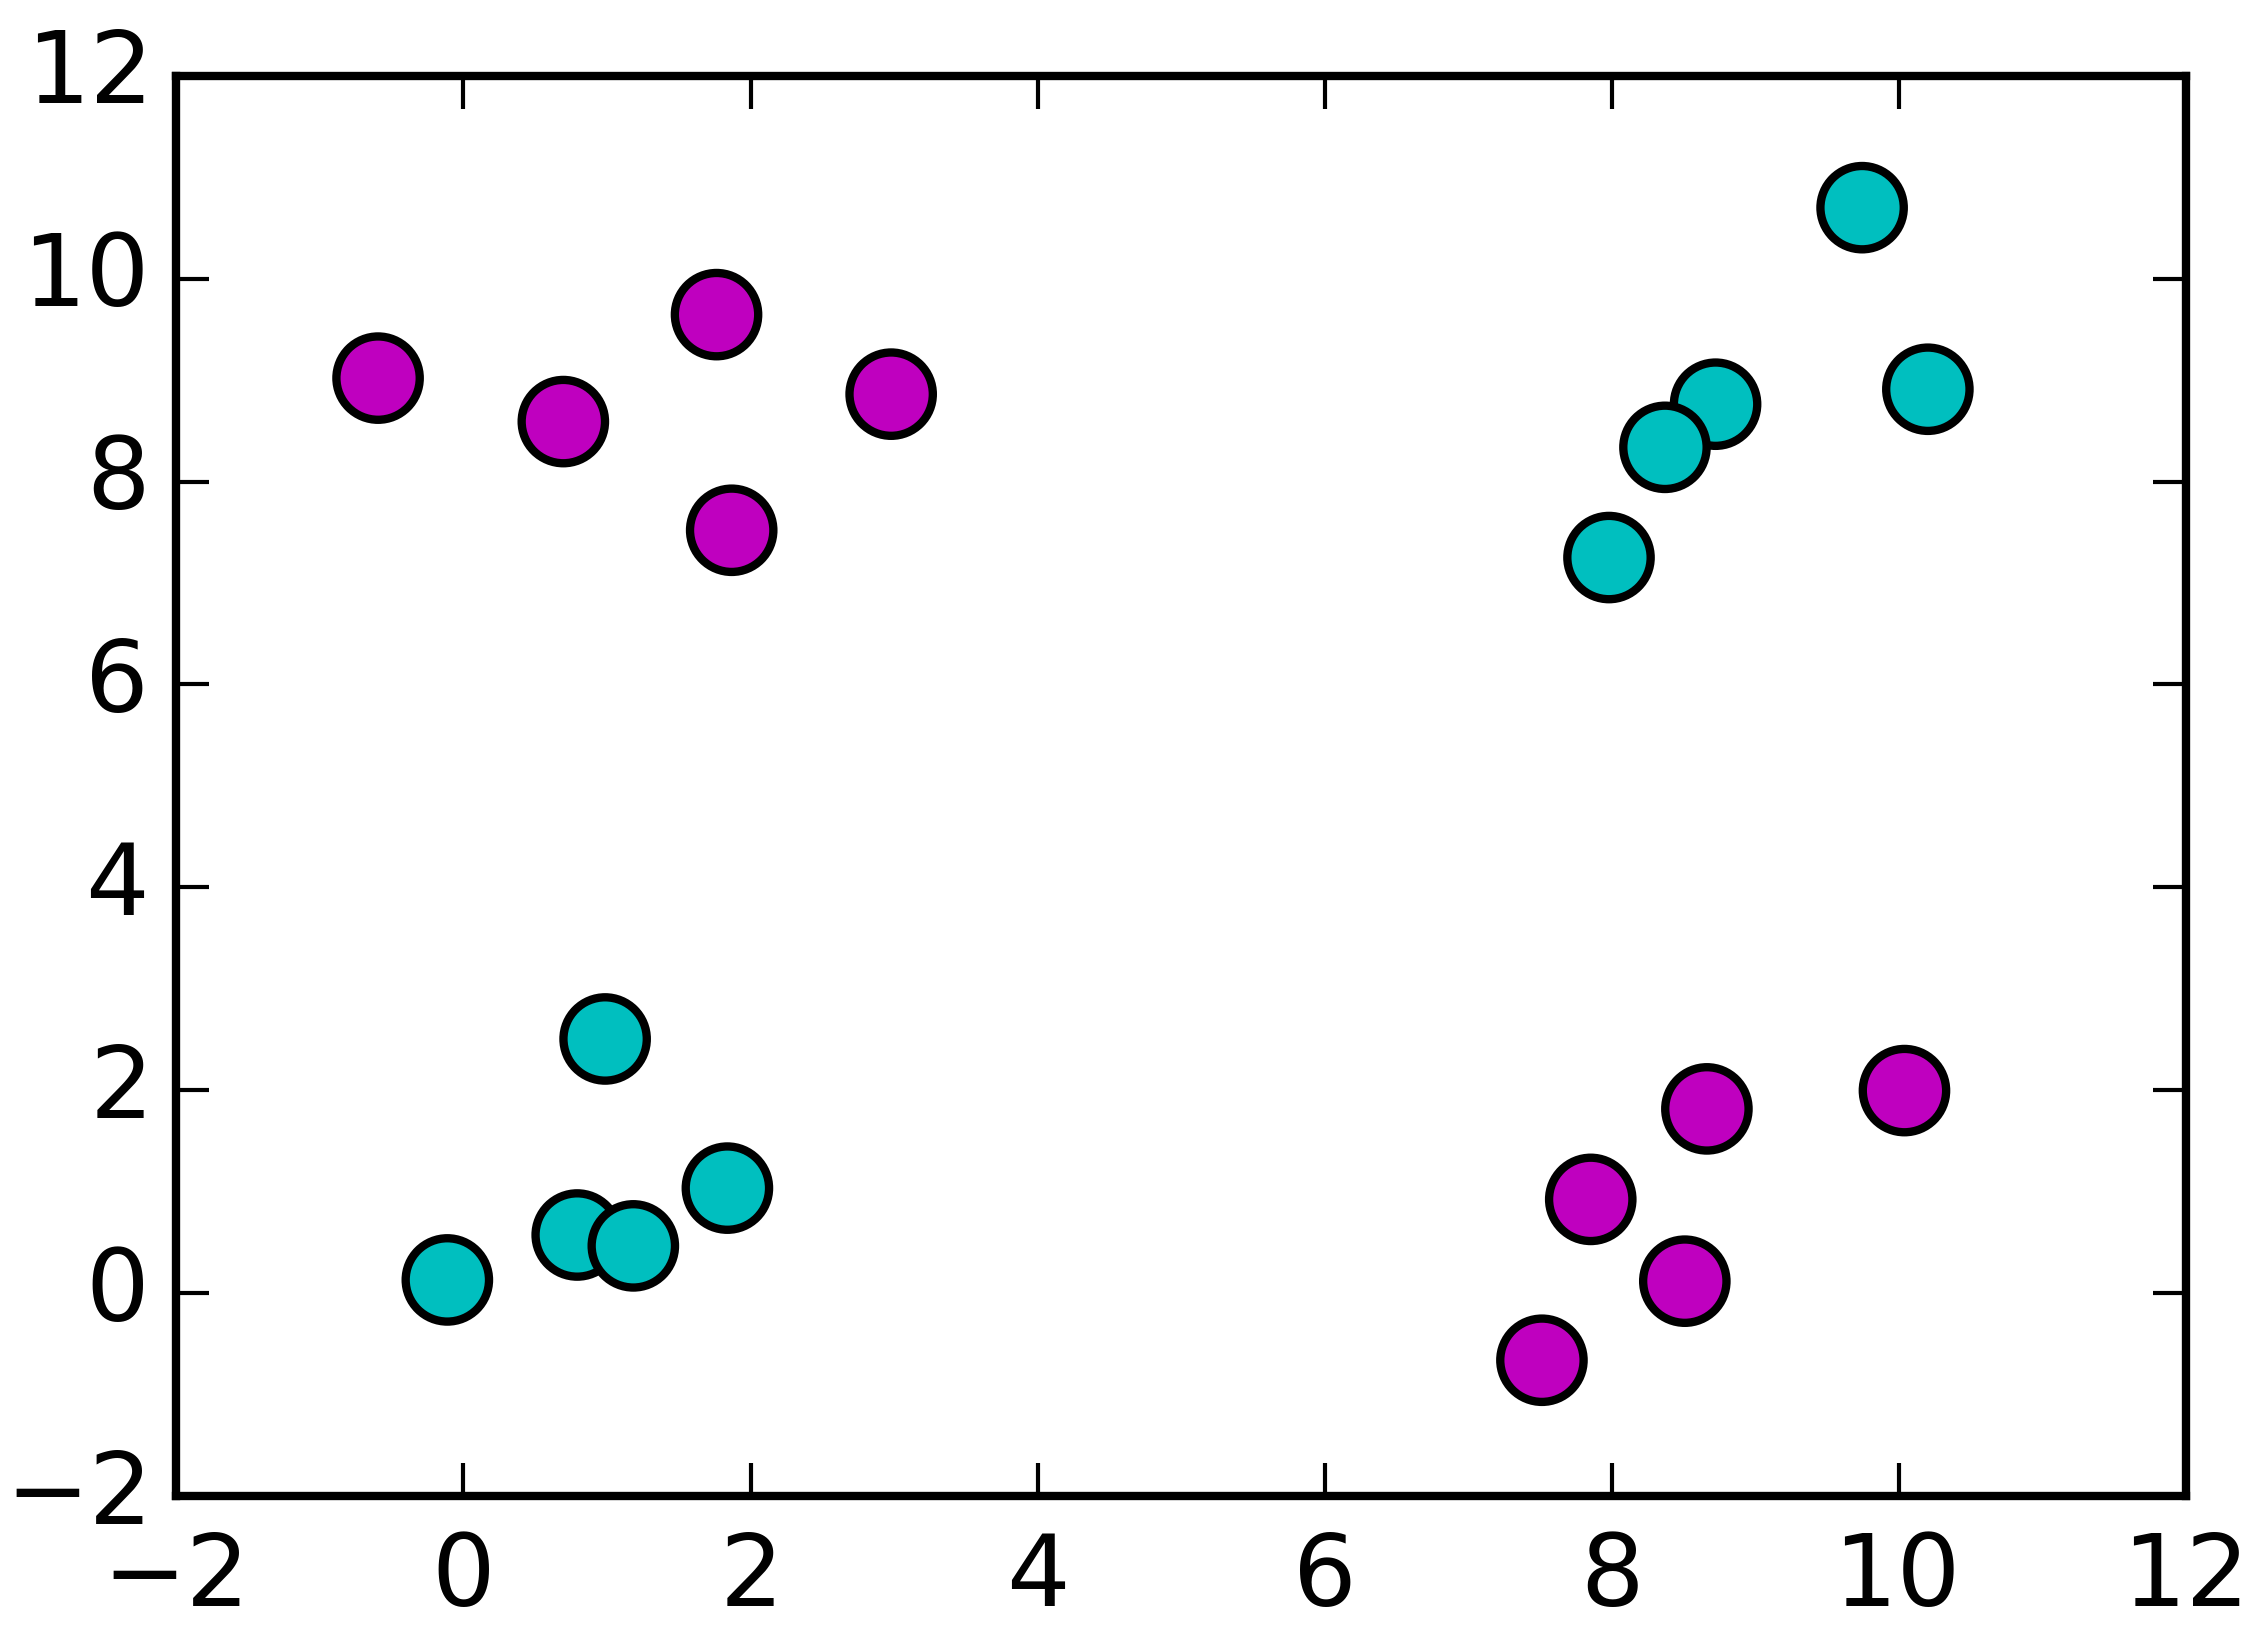
\includegraphics[width=0.25\textwidth]{quadplot1}%
	}
	\subfloat[Pairwise differences]{%
		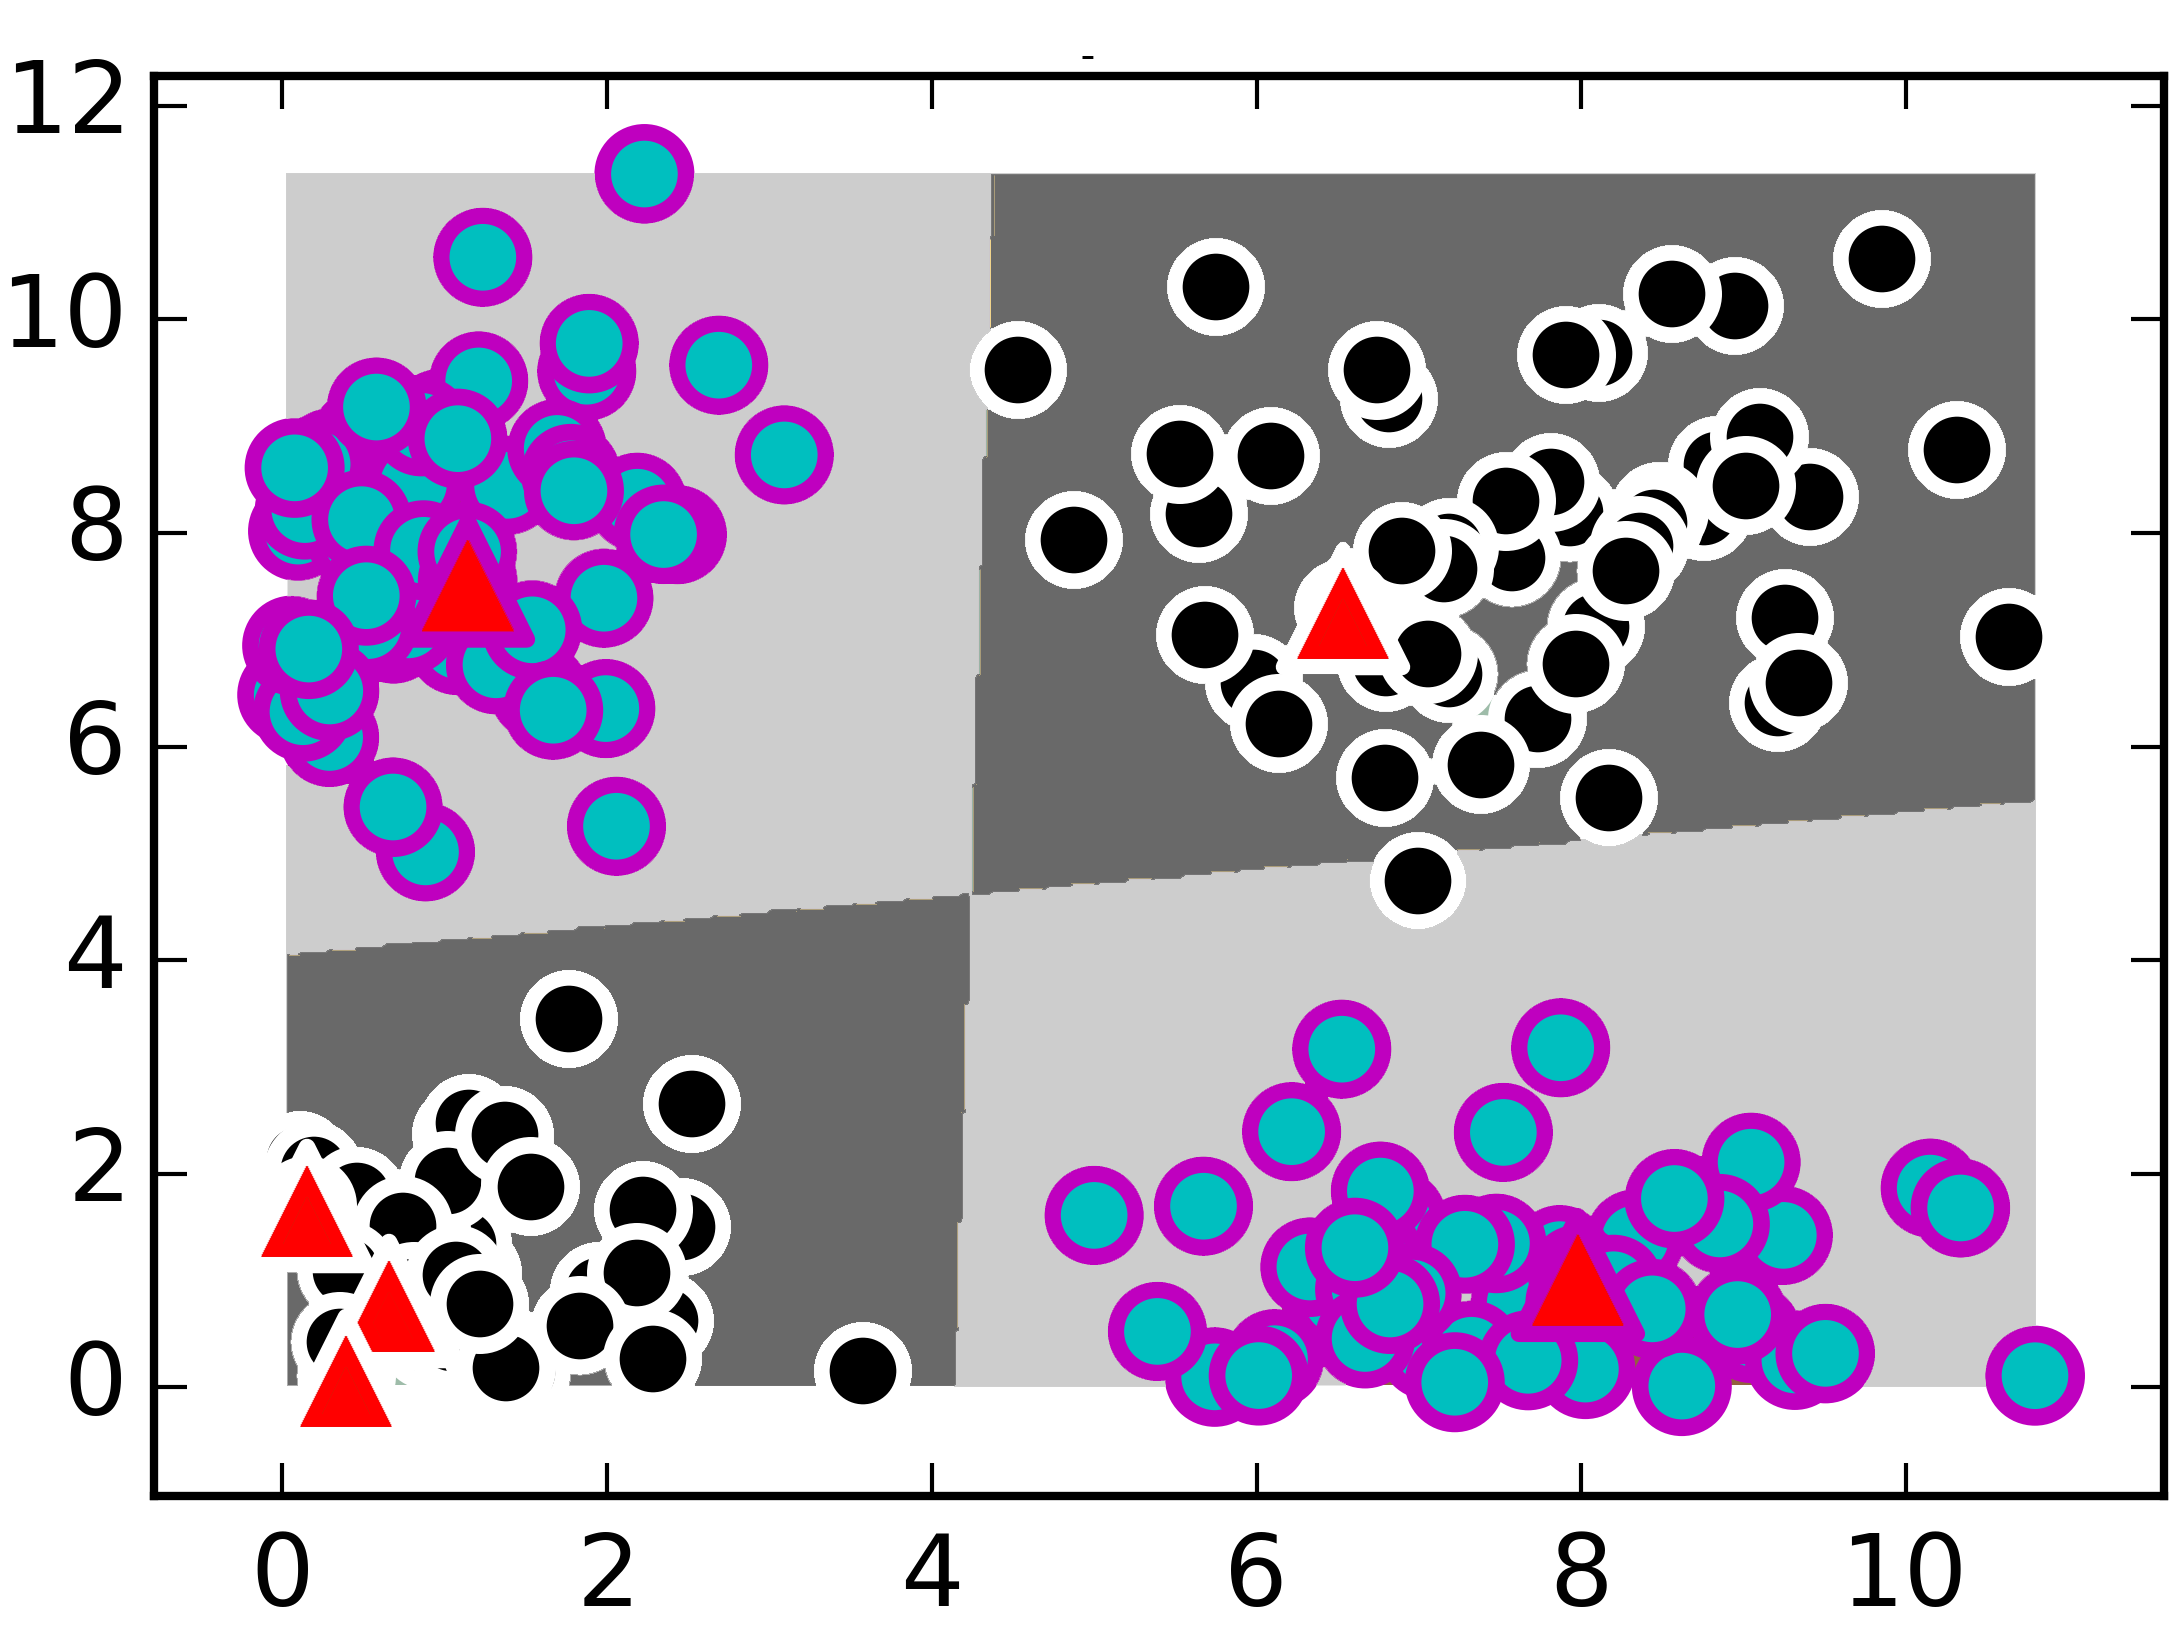
\includegraphics[width=0.25\textwidth]{quadplot2}%
	}
	\subfloat[Non-isotropic variance]{%
		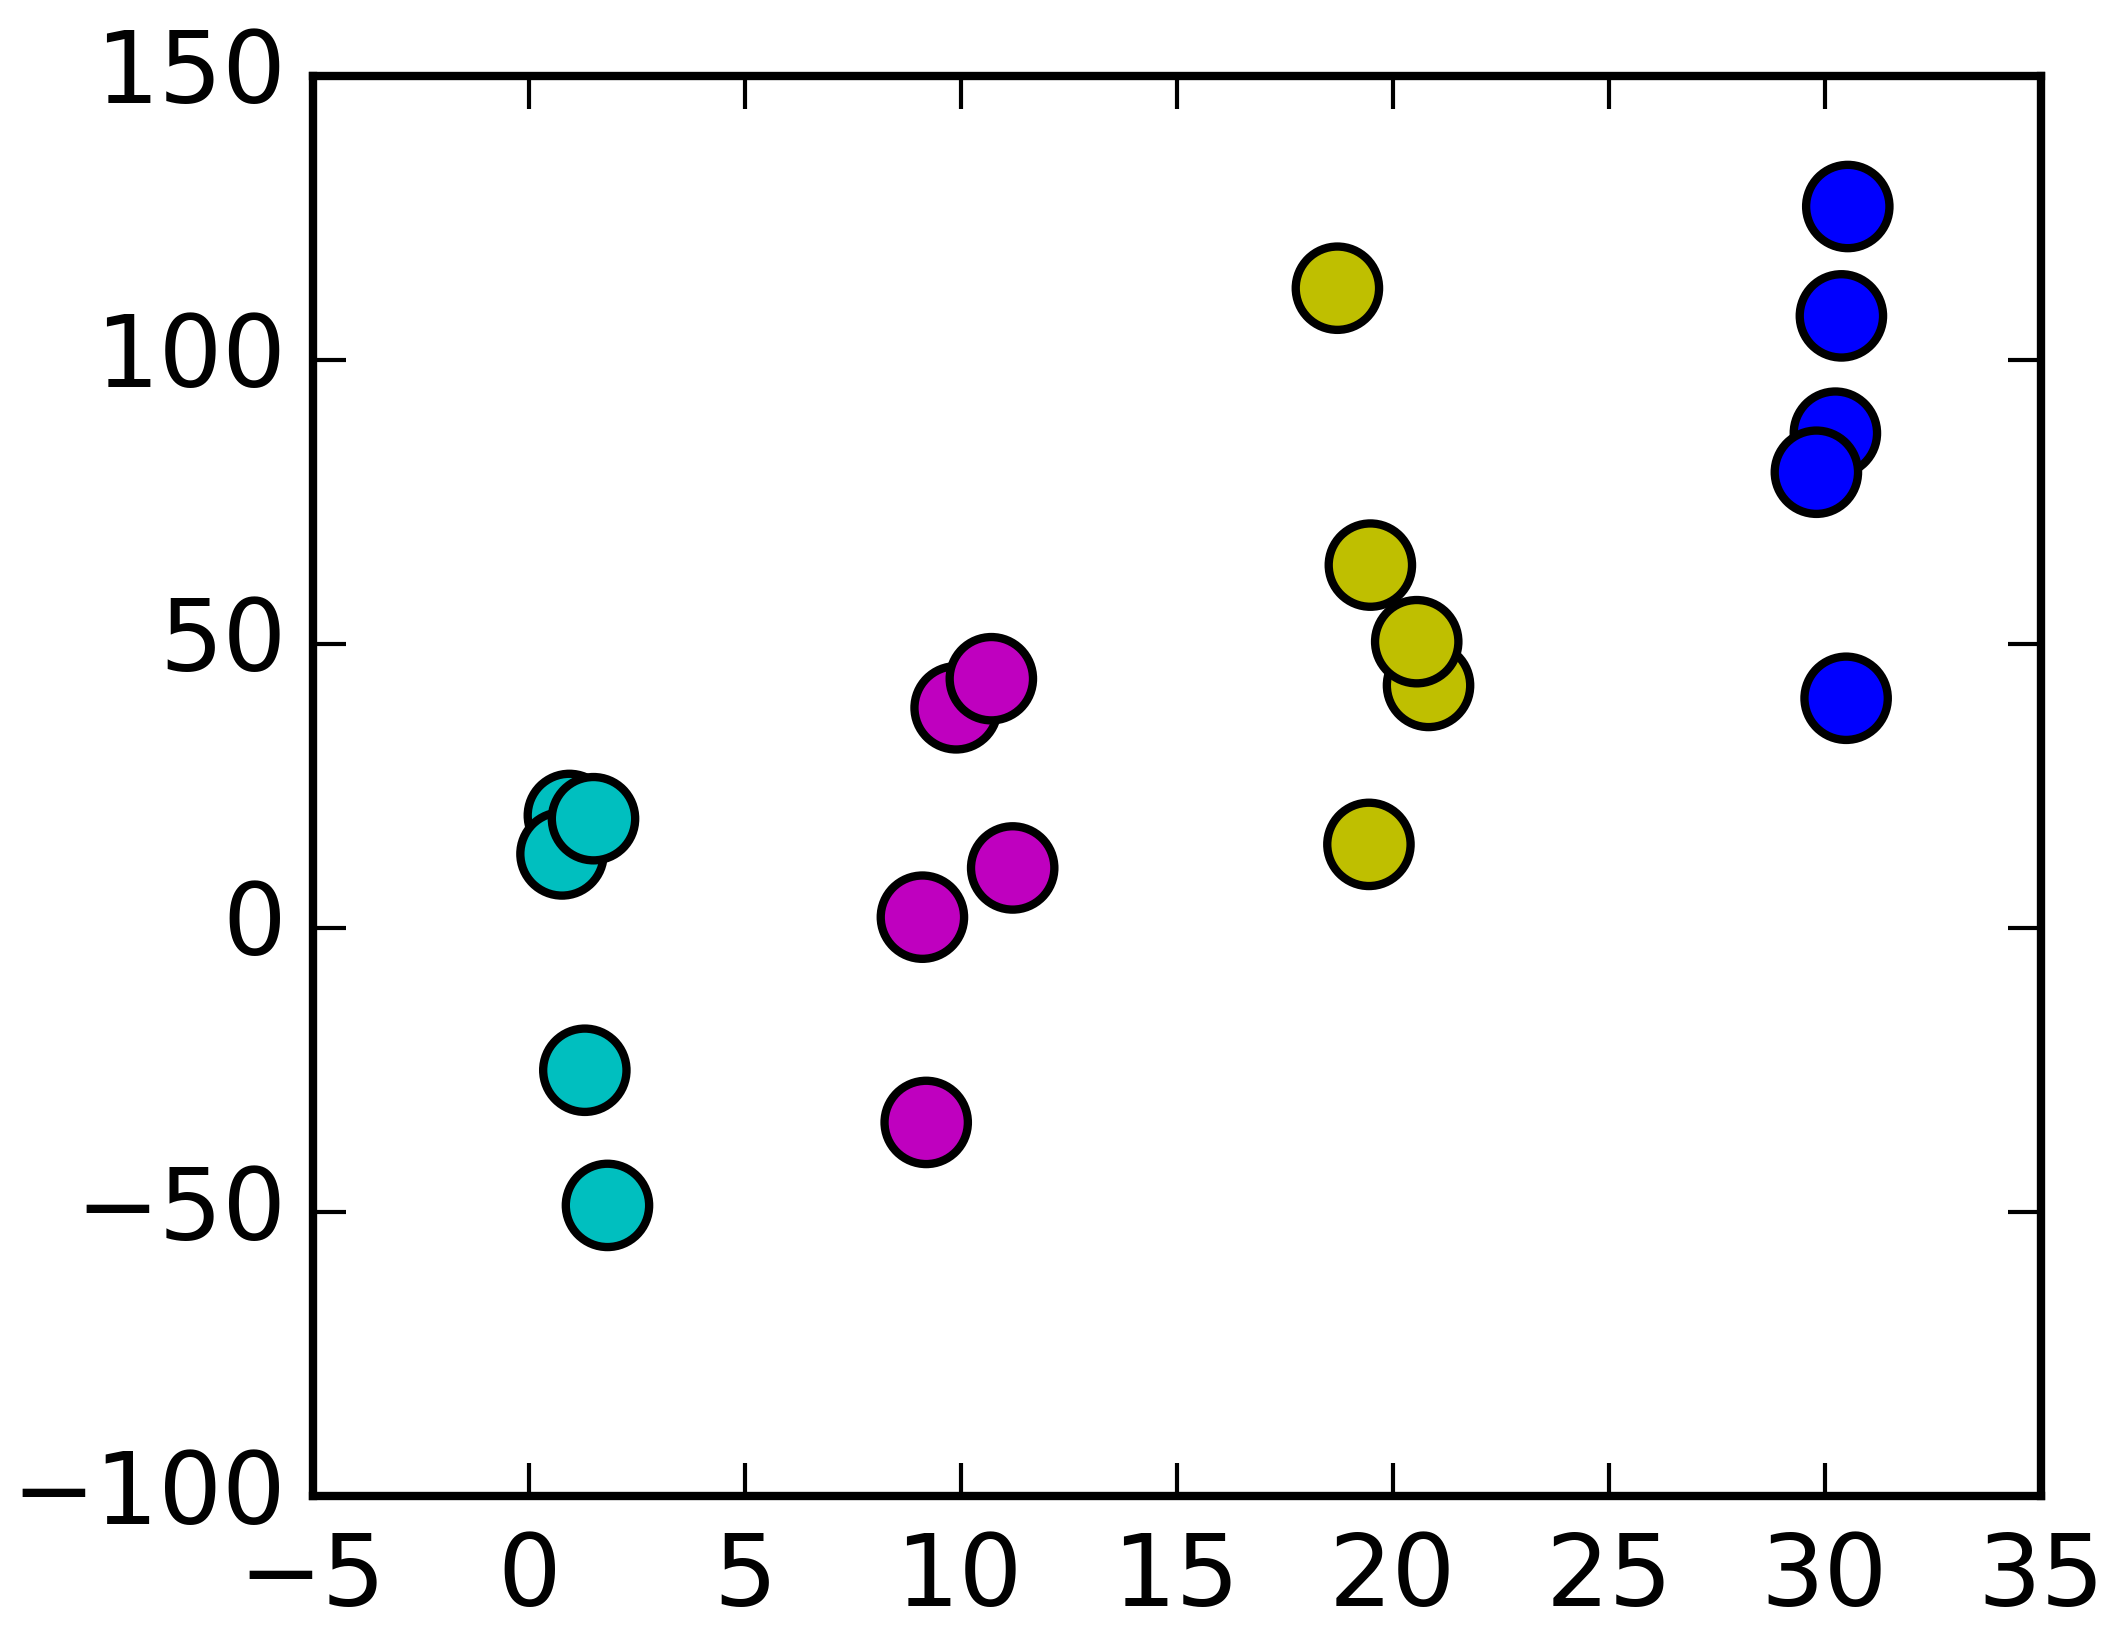
\includegraphics[width=0.25\textwidth]{isosvmproblem1}%
	}
	\subfloat[Pairwise differences]{%
		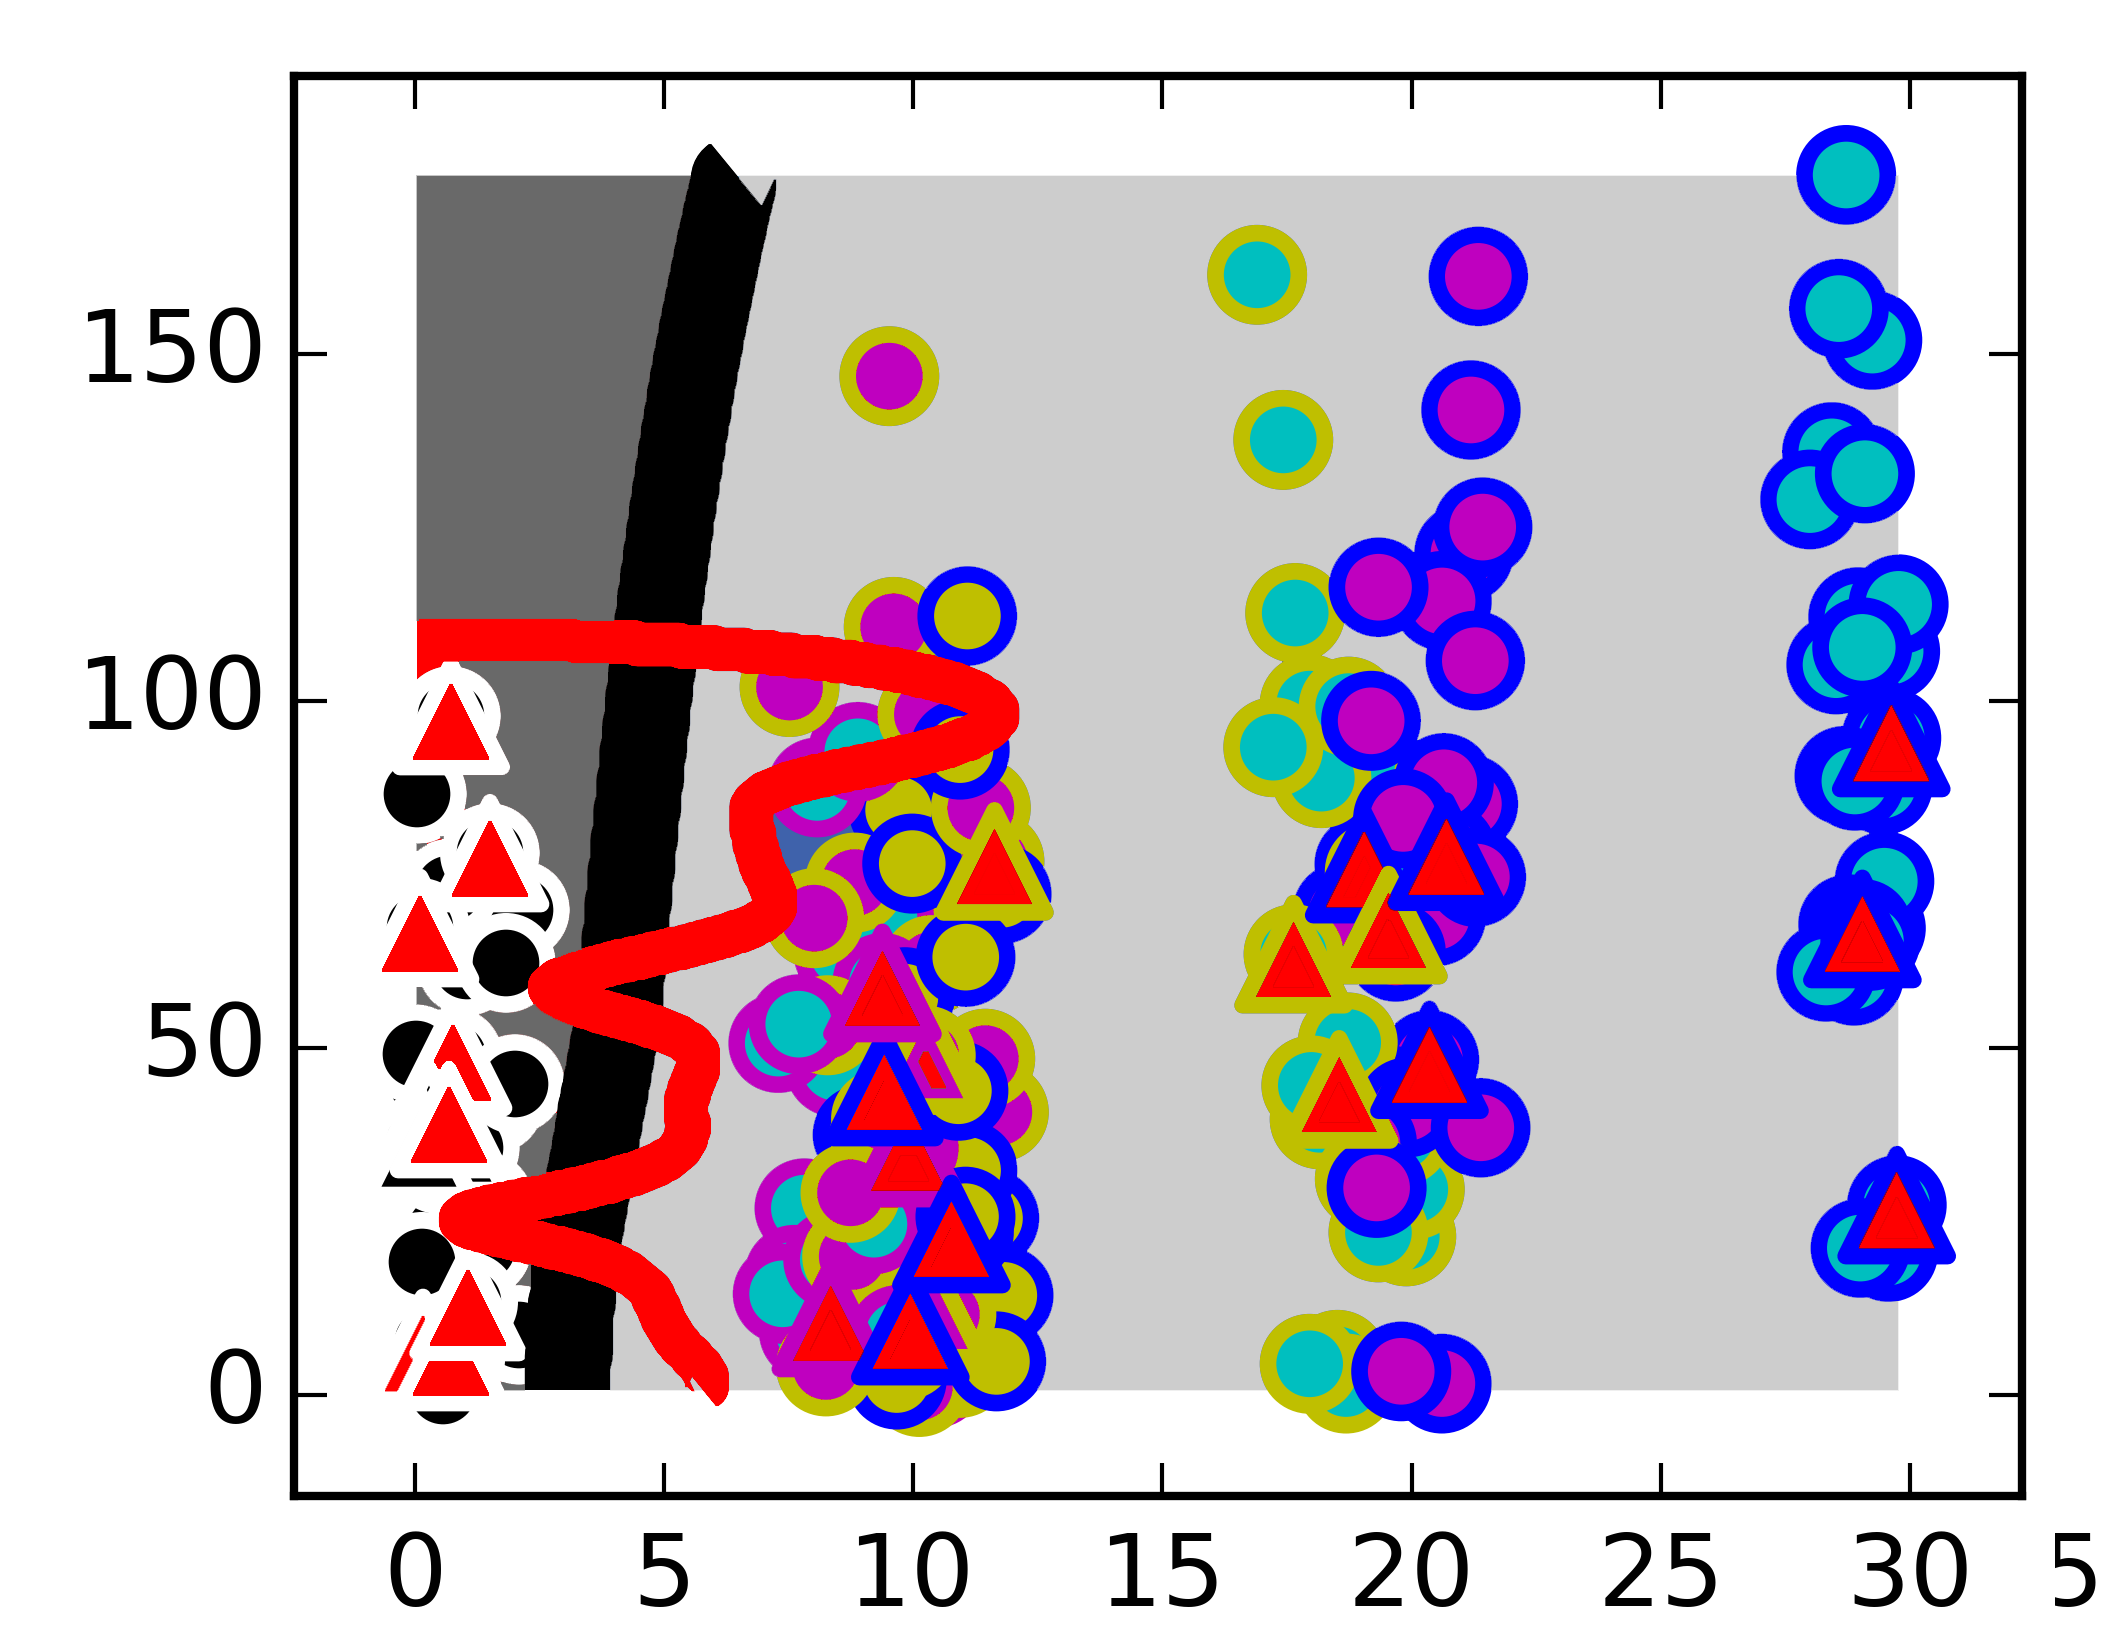
\includegraphics[width=0.25\textwidth]{isosvmproblem2}%
	}
	
	\caption[Motivation for the proposed metric learning approach]{Motivation for the proposed metric learning approach. (a) Example not linearly separable data requiring non-linear metrics. (b) Visualization of the distribution of corresponding absolute pairwise differences (APD), containing the element-wise differences in all dimensions between all possible objects, within (black) and across (coloured) clusters. The background contour shows the probability of a pair with a given distance belonging to the same cluster, learned by Gaussian Discriminant Analysis, and used as the distance pseudometric. Red triangles show the labelled ML and CL constraints. (c) Example data with non-isotropic variance (three orders of magnitude larger in the y-axis direction). (d) Corresponding APD space coloured as in (a). In addition to the modelled probability of belonging to the same cluster, the models decision boundary (black), as well as the decision boundary of a Support Vector Machine with an isotropic RBF kernel (optimal parameters set by grid search), which overfits along the low-variance dimension.}
	\label{fig:motivation}
\end{figure*}
 
Our motivations for proposing a novel non-linear method are threefold. First, we would like to sidestep the difficulty of robustly finding a good non-linear metric for a particular dataset, in a probabilistic framework, without hyperparameter tuning. Second, instead of learning a metric using an objective function based on Lp-distance, which collapses the differences along the individual dimensions into one value, we would like to let the model directly access these individual differences, and thus to learn their importance, allowing it to easily deal with non-isotropic data (Figure \ref{fig:motivation}c-d). Third, we would like to make use of prior information regarding what constitutes a `good' metric for clustering. In particular, unlike using a weighted Lp-metric which attempts to summarize the structure of within-cluster and across-cluster pairwise distances as scalars, we define \textit{a pseudo-metric based on the vector space of absolute pairwise differences} (APD). 

This not only allows straightforward learning of the importance of each feature and thus fitting non-isotropic distributions better than isotropic kernels (Figure \ref{fig:motivation}c-d), but also makes explicit the structure in the distribution of constraints. It has been observed before that for data containing clusters, the probability density function of pairwise Lp distances shows two peaks (one for within- and one for across-cluster pairs), e.g. by \citep{brin1995near}. However, in the case of multiple clusters with different shapes and variances, a bimodal distribution is insufficient to reflect the true distributions of the instance differences within or across clusters. Clearly, within-cluster variances in one cluster do not have to equal those in another cluster, and the same is true for across-cluster variances (as illustrated by the variances of the groups of data in APD space in Figure \ref{fig:motivation}b and d). Learning in pairwise difference vector space (instead of collapsing these distances into scalars) allows our model to adapt locally to within- and across-cluster variances of different clusters, and therefore to better approximate the true pairwise distance distribution. 

\section*{Supervised learning in absolute pairwise difference space}

The formulation of (weakly) supervised learning in absolute pairwise difference space was given in Chapter 2.5 above. We briefly summarize it as follows.

Let $\mathcal{X}=(\boldsymbol x_i, ..., \boldsymbol x_n)$ be the feature vector representation of $n$ objects which are to be clustered, where $x_i \in \mathbb{R}^D$ are vectors with $D$ dimensions. Let the set of $m$ given pairwise linkage constraints be denoted by $\mathcal{L}$, where $ \lvert \mathcal{L} \lvert = m $, and $l_{i,j} \in \mathcal{L}$ is

\begin{equation}
l_{i,j}=
\begin{cases}
1, & \text{if $i$ and $j$ belong to the same cluster (ML constraint)} \\
0, & \text{if $i$ and $j$ belong to different clusters (CL constraint)}
\end{cases}
\end{equation}

Then, a distance metric $d_l$ between two instances can be defined based on the probability that these instances belong to the same cluster, making use of a generative classifier (constituent model) trained on the given constraints:

\begin{equation}
\label{eq:metric}
d_l(\boldsymbol x_1, \boldsymbol x_2; \boldsymbol{\theta}) = 1 - p(l=1|\Delta \boldsymbol x, \boldsymbol{\theta}) = p(l=0|\Delta \boldsymbol x, \boldsymbol{\theta})
\end{equation}

There are three advantages of using generative classifiers instead of just the classification output as the pseudometric. First, this makes the model well-suited to learning in the inductive setting (where the examples from the test set are not seen at training time). Many existing approaches are designed for and evaluated in the transductive setting. Second, on more complex, unseparable data, utilizing the models confidence of whether instances should be linked, in addition to a binary prediction, greatly improves the resulting clustering. Finally, this choice allows choosing suitable priors and likelihoods and thus tailoring the model to fit the data at hand.

\section*{Extension of the framework to semi-supervised learning}

Given the large number of pairwise differences, ${n \choose 2}=\frac{n^2-n}{2}$, the following question arises: why only use the tiny set of given pairwise constraints for learning, instead of making use of the entire distribution in APD space?

An extension of a recently proposed framework for semi-supervised learning, called Contrastive Pessimistic Likelihood Estimation (CPLE) \citep{loog2015contrastive}, can facilitate such an approach for using the entire APD space. \cite{loog2015contrastive} points out that most current semi-supervised approaches are not `safe' (do not guarantee better performance when including the unlabelled data than without), and often perform sub-optimally due to model misspecification (making assumptions violated by data). Instead, he suggests only using the intrinsic assumptions of a given classifier, and training it in a pessimistic framework: using optimization to find hypothetical labels for the unlabelled data corresponding to the worst case. This pessimism ensures that the inclusion of unlabelled data point cannot make the model accuracy worse than just using the labelled data. 

In practice, his procedure pessimistically assign soft labels to the unlabelled data, such that the improvement over the supervised version is minimal; at the same time maximize log likelihood over labelled data. That is, the parameters $\theta_{semi}$ of a semi-supervised model in the CPLE framework are given by

\begin{equation}
\label{eq:cple}
\theta_{semi} = \argmax_\theta \argmin_q L(\theta|X,U,q) - L(\theta_{sup}|X,U,q),
\end{equation}

where $X={(x_i,y_i)}_{i=1}^N$ denotes the labelled data, $U$ the unlabelled data, and $q$ the hypothetical soft labels. \citep{loog2015contrastive} only provides a solution for Linear Discriminant Analysis (LDA), and his framework requires an explicit generative likelihood $L(\theta|X,U,q)$.

However, his framework can be modified to use discriminative likelihoods instead. This allows using both generative and discriminative classifiers in this framework, provided that they can output a prediction probability (such probability estimates can also be provided by Platt scaling \citep{platt1999probabilistic} for classifiers which don't support them). 

Figure \ref{cplealg} shows the objective function this extended CPLE model, supporting pessimistic semi-supervised learning with any constituent model. Instead of optimizing the generative likelihood $L$, the negative log loss $J(y,r)=log p(y|r)=\frac{1}{N} \sum_{i=1}^N (y_i \text{log} (r_i) + (1-y_i) \text{log} (1-r_i))$ is used in the optimization objective, where $y_i$ is the predicted class of the $i$'th instance, and $r_i$ is the probability associated with this prediction.

\begin{figure}[h]
	\begin{pseudocode}{cpleObjectiveFunction}{model, \theta, q, X, y, U}
		1: \text{set} \enspace z_i \GETS \begin{cases}
			1 & \text{if } q_i \geq 0.5\\
			0 & \text{otherwise}
		\end{cases} \enspace \text{for all} \enspace i \in [1, |U|] \\
		2: X' \GETS X \cup U \\
		3: y' \GETS y \cup z \\
		4: \text{set} \enspace w_i \GETS \begin{cases}
			1 & \text{if } X'_i \in X \\
			q_i & \text{otherwise}
		\end{cases} \enspace \text{for all} \enspace i \in [1, |X'|] \\
		5: model \GETS train(model, X', y', w) \\
		6: r \GETS predictionprobability(model, X) \\
		7: r' \GETS predictionprobability(model, U) \\
		8: J_{labelled} \GETS \frac{1}{|X|} \sum_{i=1}^{|X|} (y_i \text{log} (r_i) + (1-y_i) \text{log} (1-r_i)) \\
		9: J_{unlabelled} \GETS \frac{1}{|U|} \sum_{i=1}^{|U|} (z_i \text{log} (r'_i) + (1-z_i) \text{log} (1-r'_i)) \\
		10: return(J_{unlabelled} - J_{labelled})
	\end{pseudocode}
	\caption[Objective function for a general pessimistic semi-supervised learning framework]{\textbf{A general pessimistic semi-supervised learning framework,} based on a generalization of \citep{loog2015contrastive} to use discriminative likelihoods and to be usable with any classifier supporting prediction probabilities. It requires a constituent model, current hypothetical labels $q$ of the unlabelled data points and model parameters $\theta$ which are to be optimized, the unlabelled data $U$, labelled data $X$, labels $y$ of $X$, and the negative log loss $J_{labelled}$ of the model trained only on $X$. Minimizing this objective increases accuracy over the labelled data while assuming worst-case labels for the unlabelled data}
	\label{cplealg}
\end{figure}


The modified CPLE objective function in Figure \ref{cplealg} can be used with any global optimization approach to train a model to fit the unlabelled data distribution in a pessimistic fashion, while maximizing performance over the labelled data. We used the locally biased variant \citep{gablonsky2001locally} of DIRECT (DIviding RECTangles) \citep{jones1993lipschitzian}, a global, deterministic, derivative-free optimization method based on Lipschitzian optimization, which can handle the kinds of non-linear and non-convex functions constituted by Figure \ref{cplealg}. 

The resulting semi-supervised learning framework is highly computationally expensive, but has the advantages of being a generally applicable framework, needing low memory, and making no additional assumptions except for the ones made by the chosen classifier.

\section*{Constituent models}

%TODO derive minimum no. of constraints

In principle, any generative classification model could be used as the constituent model in \eqref{eq:metric} to model the linkage probability distribution. Here, we focus on three models of this class (NB, GDA and GP), the first two of which have closed form solutions, thus constituting the - to our knowledge - first probabilistically motivated approach to learning a non-linear distance metric in closed form.
%Thus, they facilitate the - to our knowledge - first probabilistically motivated approach to learning a non-linear distance metric in closed form. \footnote{GPs have a closed-form solution (the best linear unbiased prediction) if the autocorrelation model is known; otherwise, it can be estimated using Expectation Maximization \citep{gpml06}}. 

%TODO rewrite all this shit. use gaussian mixture model discriminant analysis. possibly use multinomial mixture model - p. 5 and 6 in http://math.univ-lille1.fr/~biernack/index_files/articleJSS.pdf
%http://www.mixmod.org/IMG/pdf/statdoc_2014.pdf
%http://www.r-bloggers.com/a-brief-look-at-mixture-discriminant-analysis/

In the case of \textbf{GDA} \citep{bensmail1996regularized}, the likelihoods of a pair of instances belonging to the same cluster $p( \Delta \textbf x | l=1; \mu_1, \Sigma_1)$ or to different clusters $p( \Delta \textbf x | l=0; \mu_0, \Sigma_0) $, are modelled using multivariate Gaussians:

\begin{equation}
\label{eq:gda}
p( \Delta \textbf x | l=i; \mu_i, \Sigma_i) = (2\pi)^{-\frac{D}{2}}|\boldsymbol\Sigma_i|^{-\frac{1}{2}}\, e^{ -\frac{1}{2}(\Delta \mathbf{x}-\boldsymbol\mu_i)^\intercal\boldsymbol\Sigma_i^{-1}(\Delta \mathbf{x}-\boldsymbol\mu_i) },
\end{equation}

where $i \in \{0,1\}$. $(\mu_1, \Sigma_1)$ are the means and covariances of the APD distances of pairs in the same cluster, and $(\mu_0, \Sigma_0)$ those in different clusters. These parameters can be easily estimated from the instances corresponding to the must-link and cannot-link constraints, respectively, by calculating their means and covariances. 

%In the case of \textbf{GDA} \citep{bensmail1996regularized}, the likelihood of a pair of instances belonging to one of the $K+A$ assumed APD distributions $\mathcal{D}_i$ (which can be either a within-cluster or across-cluster distribution),  are modelled using multivariate Gaussians: 

%\begin{equation}
%\label{eq:mvnormal}
%p( \Delta \textbf x | \Delta \textbf x \in \mathcal{D}_i; \mu_i, \Sigma_i) = (2\pi)^{-\frac{D}{2}}|\boldsymbol\Sigma_i|^{-\frac{1}{2}}\, e^{ -\frac{1}{2}(\Delta \mathbf{x}-\boldsymbol\mu_i)^\intercal\boldsymbol\Sigma_i^{-1}(\Delta \mathbf{x}-\boldsymbol\mu_i) }
%\end{equation}

%, and estimated from the given sets of must-link and cannot-link constraints $\mathcal{L}^{ML}_k \in \mathcal{L}$ and $\mathcal{L}^{CL}_k \in \mathcal{L}$

%$(\mu_i, \Sigma_i)$ are the means and covariances of the APD distances of $\Delta \boldsymbol{x}_j \in \mathcal{L}^{ML}_k$ for $\mathcal{D}=\mathcal{W}$, and of $\Delta \boldsymbol{x}_j \in \mathcal{L}^{CL}_k$ for $\mathcal{D}=\mathcal{A}$, and can be calculated analytically. The priors $p(\Delta \textbf x \in \mathcal{D}_i)=\frac{1}{m} |\mathcal{L}_i|$ simply reflect the relative frequency of the constraints in the relevant subset.

In the case of \textbf{GP}, we model the linkage probability distribution using a Gaussian Process with mean function $m(\cdot)$ and covariance function $k(\cdot)$:  

% linear kernel - actually doing Bayesian linear regression, can be done in O(n)! Try scikits' BayesianRidge and/or Ridge Classifier http://people.seas.harvard.edu/~dduvenaud/cookbook/

\begin{equation}
\label{eq:gp}
p(\Delta \textbf x | l=i; M, K) = \mathcal{GP}(m(\cdot), k(\cdot)) = \mathcal{N}\Bigg( \begin{bmatrix}m(x_1) \\ \vdots \\ m(x_m) \end{bmatrix},  \begin{bmatrix}k(x_1, x_1), ..., k(x_1, x_m) \\ \vdots \quad \quad \ddots \quad \quad \vdots \\ k(x_m, x_1), ..., k(x_m, x_m)\end{bmatrix}  \Bigg)
\end{equation}

In the experiments below, we have used a zero mean function and the square exponential kernel as the covariance function. See \citep{rasmussen2005gp} for an extensive book on Gaussian Processes.

For Multinomial \textbf{Naive Bayes} \citep{kibriya2005multinomial}, which is suitable for e.g. text data, the likelihood given $K$ event counts (e.g. word counts) is simply

\begin{equation}
\label{eq:nb}
p(\Delta \textbf x | l=i; \Phi_{0}, \Phi_{1}) = \frac{(\sum_j \Delta x_j)!}{\prod_j \Delta x_j!} \prod_j p_{ij}^{\Delta x_j},
\end{equation}

where $p_{ij}$ are the probabilities that word $j$ occurs within ($i=1$) or across ($i=0$) a cluster of documents, estimated from the provided constraints. The feature vectors $x$, instead of just traditional word frequencies, are calculated using term frequency and inverse document frequency for each word, as suggested by \citep{rennie2003tackling}.

\section*{Preliminary results}

We will first assume a purely supervised case - plugging in a GDA model (Equation \eqref{eq:gda}) into the APD metric framework (Equation \eqref{eq:metric}), as used to model human spatial representation structure in Chapters 2.5 and 5. We have claimed in Chapter 2.5 that our metric is well-suited for clustering, in the sense that for most within-cluster differences $\Delta \boldsymbol x_r$ and across-cluster differences $\Delta \boldsymbol x_n $ it holds that $ d_r(\boldsymbol x_{r,1}, \textbf x_{r,2}; \boldsymbol{\theta}) < d_n(\boldsymbol x_{n,1}, \textbf x_{n,2}; \boldsymbol{\theta}) $. 

Figure \ref{embedding} shows distances under our metric in three example datasets, embedded into two dimensions for visualization using MDS. It contrasts these distances with embeddings by t-SNE \citep{van2008visualizing}, a state of the art method for visualization, designed to represent high-dimensional data points in such a way that similar objects are modelled by nearby points, and dissimilar objects by distant points. Figure \ref{embedding} shows that the APD metric `pulls together' different clusters (shown using different colours) more effectively than t-SNE. 

The Figure is intended to show that datasets with no clear intrinsic cluster structure can be made separable by learning in APD space given only a few pairwise constraints (20 in these examples, which is less than $0.1 \%$ of all pairwise constraints), even with a fully supervised constituent model. It is not intended as a fair comparison, as t-SNE is an unsupervised method.

\begin{figure*}[t]
	\centering
	
	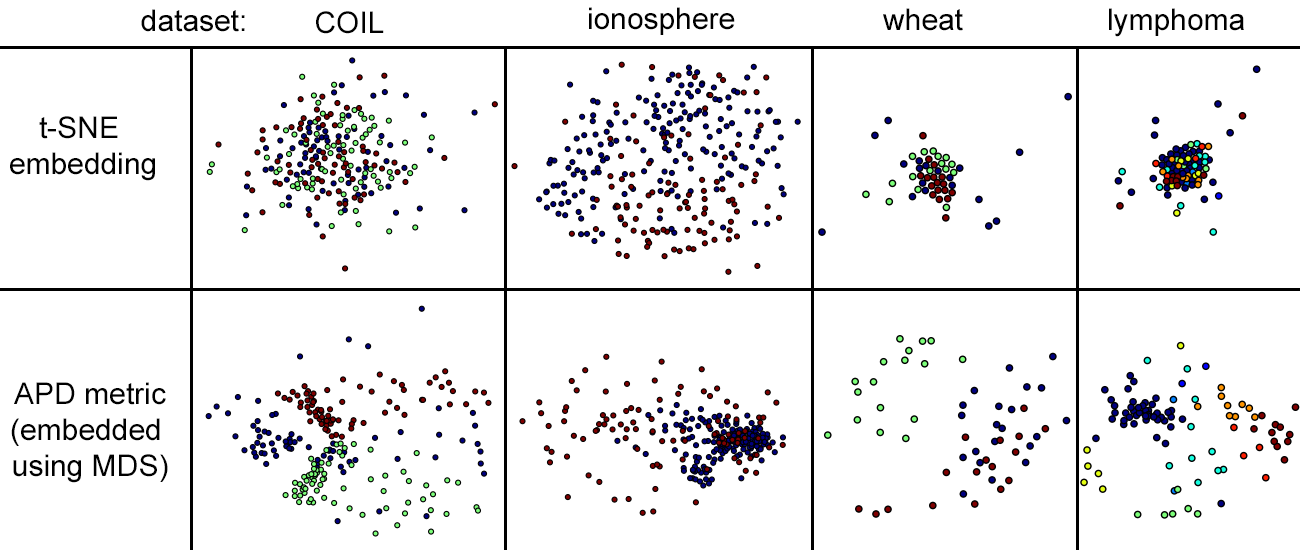
\includegraphics[width=\textwidth]{embeddingresults}%
	
	\caption[Embedding of pairwise distances as suggested by our metric learning approach]{Embedding of pairwise distances as suggested by our metric learning approach (top) and by t-SNE (bottom) on the COIL-3 dataset (128x128px images of 3 similar-looking toy cars) used by \citep{zeng2012semi}, the ionosphere and wheat datasets from the UCI machine learning repository, and the lymphoma microarray dataset obtained from the Broad Institute. The APD plot was created using supervised GDA as the constituent model.}
	\label{embedding} 
\end{figure*}


\subsection*{Clustering results - semi-supervised constituent models}

\begin{tabularx}{\textwidth}{|*{8}{c|}}
	\cline{1-8}
	\begin{tabular}[c]{@{}c@{}} \text{data-}\\\text{set} \end{tabular} & \begin{tabular}[c]{@{}c@{}} \text{cons-}\\\text{traints} \end{tabular} & \begin{tabular}[c]{@{}c@{}} \text{DCA+}\\\text{KMeans} \end{tabular} & \text{Kmeans} & \begin{tabular}[c]{@{}c@{}} \text{MPC}\\\text{KMeans} \end{tabular} & \begin{tabular}[c]{@{}c@{}} \text{SS-}\\\text{MMC} \end{tabular} & \begin{tabular}[c]{@{}c@{}} \textbf{ADS-}\\\textbf{GDA} \end{tabular} & \begin{tabular}[c]{@{}c@{}} \textbf{ADS-}\\\textbf{LS} \end{tabular} \\ \cline{1-8}
	\multirow{5}{*}{\begin{tabular}[c]{@{}c@{}} \text{pen}\\\text{digit} \end{tabular}}  & 20 & 0.318 & 0.545 & 0.541 & 0.666 & 0.427 & \textbf{0.821} \\
	& 40 & 0.328 & 0.545 & 0.556 & 0.743 & 0.554 & \textbf{0.874} \\
	& 60 & 0.553 & 0.545 & 0.535 & 0.831 & 0.717 & \textbf{0.855} \\ 
	& 80 & 0.677 & 0.545 & 0.58 & 0.833 & 0.769 & \textbf{0.901} \\ 
	& 100 & 0.721 & 0.545 & 0.537 & 0.861 & 0.8 & \textbf{0.878} \\ \cline{1-8}
	\multirow{5}{*}{\begin{tabular}[c]{@{}c@{}} \text{letter}\\\text{IJL} \end{tabular}} & 20 & 0.178 & 0.266 & 0.217 & \textbf{0.447} & 0.14 & 0.337 \\ 
	& 40 & 0.207 & 0.266 & 0.223 & \textbf{0.546} & 0.194 & 0.467 \\ 
	& 60 & 0.352 & 0.266 & 0.226 & \textbf{0.691} & 0.3 & 0.431 \\ 
	& 80 & 0.4 & 0.266 & 0.167 & \textbf{0.568} & 0.417 & 0.329 \\ 
	& 100 & 0.582 & 0.266 & 0.211 & \textbf{0.655} & 0.517 & 0.571 \\ \cline{1-8}
	\multirow{5}{*}{\begin{tabular}[c]{@{}c@{}} \text{vehi}\\\text{cle} \end{tabular}} & 50 & 0.083 & 0.186 & 0.12 & 0.207 & 0.094 & \textbf{0.245} \\ 
	& 100 & 0.233 & 0.186 & 0.122 & \textbf{0.277} & 0.161 & 0.208 \\ 
	& 150 & 0.331 & 0.186 & 0.122 & \textbf{0.365} & 0.248 & 0.215 \\ 
	& 200 & 0.418 & 0.186 & 0.102 & \textbf{0.411} & 0.355 & 0.288 \\ 
	& 250 & 0.459 & 0.186 & 0.113 & \textbf{0.458} & 0.351 & 0.26 \\ \cline{1-8}
	\multirow{5}{*}{\begin{tabular}[c]{@{}c@{}} \text{iono}\\\text{sphere} \end{tabular}} & 20 & 0.167 & 0.135 & 0.112 & 0.148 & 0.075 & 0.17 \\ 
	& 40 & 0.205 & 0.135 & 0.101 & \textbf{0.242} & 0.181 & 0.174 \\ 
	& 60 & 0.167 & 0.135 & 0.094 & \textbf{0.304} & 0.293 & 0.148 \\ 
	& 80 & 0.197 & 0.135 & 0.078 & 0.297 & \textbf{0.332} & 0.216 \\ 
	& 100 & 0.199 & 0.135 & 0.094 & 0.313 & \textbf{0.419} & 0.282 \\ \cline{1-8}
\end{tabularx}


%An appendix is just like any other chapter, except that it comes after
%the appendix command in the master file.
%
%One use of an appendix is to include an example of input to the system
%and the corresponding output.
%
%One way to do this is to include, unformatted, an existing input file. 
%You can do this using \verb=\verbatiminput=. In this appendix we
%include a copy of the C file \textsf{hello.c} and its output file
%\textsf{hello.out}. If you use this facility you should make sure that
%the file which you input does not contain \texttt{TAB} characters,
%since \LaTeX\ treats each \texttt{TAB} as a single space; you can use
%the Unix command \texttt{expand} (see manual page) to expand tabs into
%the appropriate number of spaces. 
%
%\section{Example input and output}
%\label{sec:inp-eg}
%\subsection{Input}
%\label{sec:input}
%(Actually, this isn't input, it's the source code, but it will do as
%an example)
%
%\verbatiminput{hello.c}
%
%\subsection{Output}
%\label{sec:output}
%
%\verbatiminput{hello.out}
%\subsection{Another way to include code}
%You can also use the capabilities of the \texttt{listings} package to
%include sections of code, it does some keyword highlighting.
%
%\lstinputlisting[language=C]{hello.c}

\bibliography{LPSP}


\end{document}
